\documentclass[12pt, a4paper, brazil, portuguese]{article}

\usepackage[margin=2.2cm]{geometry}

\usepackage[utf8]{inputenc}
\usepackage[hidelinks]{hyperref}
\usepackage{amsmath}
\usepackage{amsfonts}
\usepackage{amssymb}
\usepackage{graphicx}
\usepackage{caption}
\usepackage{subcaption}
\usepackage{sidecap}

\renewcommand{\figurename}{Figura}
\renewcommand{\tablename}{Tabela}

\renewcommand\refname{Referências}
\title{Trabalho Prático 2: Deep Learning}
\date{Junho de 2014}
  \author{
    André Taiar      \emph{taiar@dcc.ufmg.br}   \\
    João Paulo Brum  \emph{jpbrum@dcc.ufmg.br}  \\
    Philipe Melo     \emph{philipe@dcc.ufmg.br}
  }
\begin{document}

\maketitle

\section{Convolutional Neural Networks}
\subsection{Questões teóricas}
\paragraph{1} Explique o que são e para que servem cada um dos seguintes conceitos, no contexto de
  \emph{CNNs}:
\begin{itemize}
  \item Feature Map:
  \item Kernel:
  \item Convolution:
  \item Pooling:
  \item O step-size usado na implementação:
\end{itemize}

\paragraph{2} \emph{CNNs} tipicamente possuem 4 tipos de camadas: Uma camada de entrada, uma ou mais
  camadas de convolução, uma ou mais ``camadas escondidas'', e uma camada de saída. Explique a
  função que cada qual possui, e associe isto com seu padrão de conectividade.

\paragraph{3} O termo \emph{kernel} em \emph{CNNs} refere ao conjunto de pesos aplicados nas
  entradas dos \emph{feature maps}. Este termo também aparece em outros modelos, como, por exemplo,
  o \emph{SVM}. Neste caso particular, de que forma estes dois conceitos são similares? Qual é a
  significância do \emph{kernel} na classificação de um \emph{CNN}?

\subsection{Experimento: Deslocamento }
\subsection{Experimento: Aprendendo a aprender}
\subsection{Experimento: \emph{CNN} vs \emph{MLP}}

Para este experimento, compilamos e executamos o programa como foi fornecido (treinando e testando
todo o conjunto de imagens fornecidas). Fizemos a execução utilizando 30 épocas e repetimos os
testes 8 vezes para obter um desvio padrão. Executamos o programa desta forma para gerar os CNNs:

\begin{verbatim}
./cnn 2 13 5 5 5 2 2 1 100 30
\end{verbatim}

E executamos desta forma para os MLPs:

\begin{verbatim}
./cnn 0 1 100 30
\end{verbatim}

Um script chamado src\//3\_4\_cnn\_vs\_mlp.sh foi criado afim de automatizar a execução do programa
e a obtenção dos dados gerados. O gráfico das Acurácias médias nas execuções por Épocas e seu desvio
padrão para ambos os casos pode ser visto no gráfico da figura ~\ref{fig:cnn_mlp}.

\begin{figure}
  \centering
  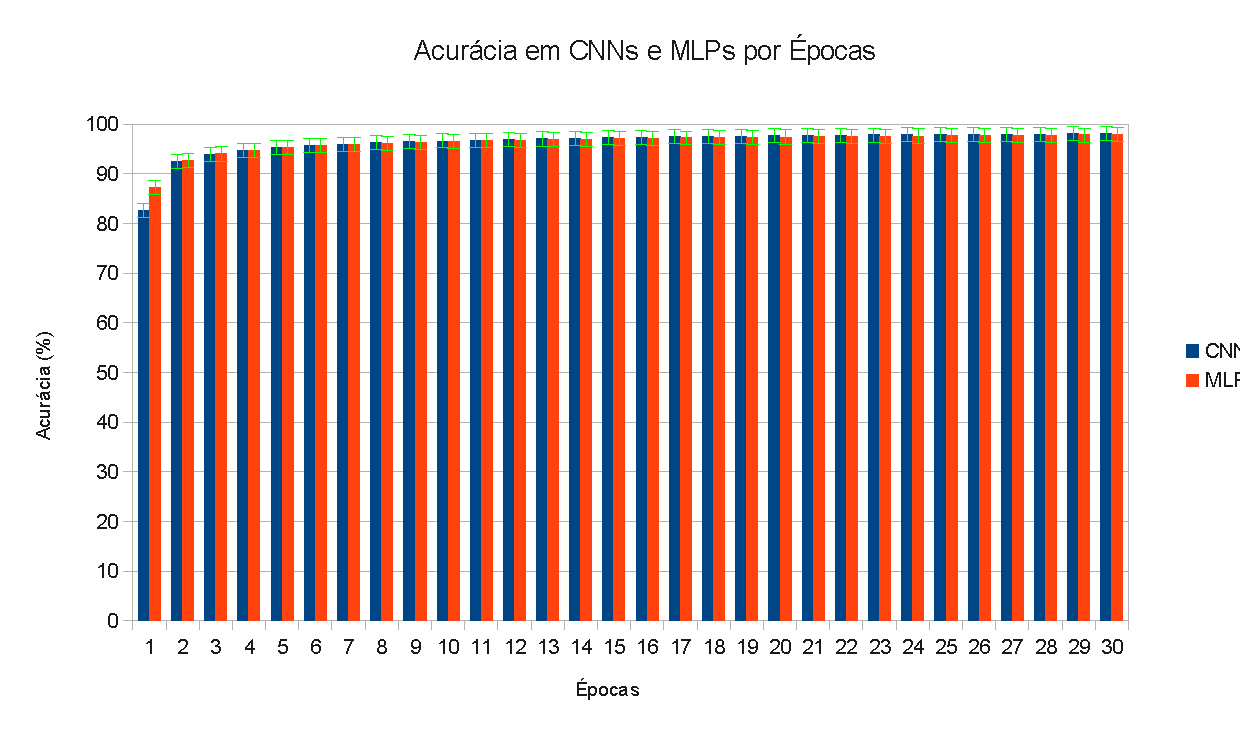
\includegraphics[width = \textwidth]{gra.pdf}
  \caption{Gráfico de Acurácia por Épocas usando CNN e MLP}
  \label{fig:cnn_mlp}
\end{figure}

Na tabela ~\ref{tab:testes_um} podem ser vistas as Acurácias médias e seus desvios padrões obtidos
nos testes.
\begin{table}
  \begin{tabular}{ c c  c  c  c }
    Classe & Acur. CNN (\%) & Desvio Padrão CNN & Acur. MLP (\%) & Desvio Padrão MLP \\
    \hline
    0 & 99.0055 & 1.4142 & 98.4563 & 1.4142 \\
    1 & 99.2730 & 1.4142 & 98.8548 & 1.4142 \\
    2 & 97.6381 & 1.4142 & 96.6931 & 1.4142 \\
    3 & 97.5497 & 1.4142 & 97.4631 & 1.4142 \\
    4 & 97.7213 & 1.4142 & 96.7287 & 1.1726 \\
    5 & 97.5197 & 1.4142 & 95.5018 & 1.2247 \\
    6 & 97.8210 & 1.4142 & 97.7426 & 1.4142 \\
    7 & 96.4613 & 1.4142 & 94.9172 & 1.4142 \\
    8 & 97.9723 & 1.4142 & 96.8686 & 1.4142 \\
    9 & 96.9028 & 1.1726 & 96.1350 & 1.4142 \\
  \end{tabular}
  \caption{Tabela de Acurácia nos testes}
  \label{tab:testes_um}
\end{table}

































\section{Stacked Denoising Auto-Encoders}
\subsection{Questões teóricas}
\subsection{Experimento: Valores latentes}
\subsection{Classifique}


\section{Tarefas Opcionais}
% NO SUBSECTION TILL YOU MADE IT
%
% \section{Convolutional Neural Networks}
%
% O código fonte fornecido\footnote{Agradece-se a Ishtiaq Khan, e originalmente a Mike Oneill pelo código original} implementa um \emph{CNN} em C++. Ele consiste em um programa funcional, capaz de ler a base de dados do \emph{MNist}, e o classificar usando a arquitetura especificada.
%
% Sugere-se que, antes de iniciar suas alterações sobre o código, você certifique que você consegue compilar e executar-lo com os parâmetros colocados abaixo.
%
% O modelo base para \emph{Convolutional Neural Networks} que será utilizado é o proposto em \cite{citeCNN} por LeCun, expressa pela seguinte arquitetura:
% \begin{itemize}
% \item Uma camada de entrada
% \item Duas camadas convolucionais
  % \begin{itemize}
    % \item Ambas as camadas usam \emph{pooling}, implementado usando um \emph{step} de tamanho 2.
    % \item A primeira camada possui 13 \emph{feature maps}, a segunda 5.
    % \item Ambas as camadas usam \emph{kerneis} quadrados de lado 5.
  % \end{itemize}
% \item Uma camada escondida de 100 unidades completamente conectadas
% \item Uma camada de saída, com um neurônio para cada classe (10, no caso)
% \end{itemize}
%
% O formato de chamada do programa de exemplo (\emph{main.cpp}) para classificar a base do \emph{MNist} é genericamente:
% \begin{verbatim}
    % ./CNN [convolution layer count N] N*[Feature map counts]
        % N*[Kernel sizes] N*[Step sizes] [hidden layer count M]
        % M*[unit counts] [epochs]
% \end{verbatim}
%
% Onde:
% \begin{itemize}
  % \item \emph{Feature map counts}, \emph{Kernel sizes} e \emph{Step sizes} são parâmetros específicos a cada camada convolucional, que especificam a arquitetura do \emph{CNN} (consulte as referências para compreender seus significados específicos).
  % \item \emph{unit counts} é o número de unidades em cada camada escondida
  % \item \emph{epochs} é o número de vezes que o modelo passará completamente pelos dados de entrada (refinando seus pesos a cada iteração).
% \end{itemize}
%
% Em particular, para treinar o modelo de LeCun sobre os dados de entrada 10 vezes (épocas) tem-se:
  % ./CNN 2 13 5 5 5 2 2 1 100 10
% \end{verbatim}
%
% Note que podemos testar um \emph{MLP} usando a mesma implementação, com a chamada:
% \begin{verbatim}
  % ./CNN 0 1 100 10
% \end{verbatim}
%
% \subsection{Questões teóricas}
%
% \begin{enumerate}
% \item Explique o que são e para que servem cada um dos seguintes conceitos, no contexto de \emph{CNNs}: (1) Feature Map, (2) Kernel, (3) Convolution, (4) Pooling, (5) O step-size usado na implementação
% \item \emph{CNNs} tipicamente possuem 4 tipos de camadas: Uma camada de entrada, uma ou mais camadas de convolução, uma ou mais ``camadas escondidas'', e uma camada de saída. Explique a função que cada qual possui, e associe isto com seu padrão de conectividade.
% \item O termo \emph{kernel} em \emph{CNNs} refere ao conjunto de pesos aplicados nas entradas dos \emph{feature maps}. Este termo também aparece em outros modelos, como, por exemplo, o \emph{SVM}. Neste caso particular, de que forma estes dois conceitos são similares? Qual é a significância do \emph{kernel} na classificação de um \emph{CNN}?
% \end{enumerate}
%
%
% \subsection{Experimento: Deslocamento }
%
% Nesse experimento, pede-se o seguinte:
% \begin{enumerate}
% \item Crie um novo \emph{CNN} que aceite como entrada os dados do \emph{MNist}, porém que tenha uma primeira camada convolucional com um único \emph{Feature Map} de largura 25 (ou seja, com um kernel de largura 4).
% \item Sem precisar treinar, aplique uma entrada qualquer do conjunto de treino na rede, e extraia o valor atingido pelos neurônios na camada convolucionária (definida no primeiro item). Plote este resultado em um mapa de calor e o insira aqui.
% \item Altere a entrada de tal forma que todos os pixels são deslocados para a direita por 5 posições, e repita o procedimento anterior, inclusive o plot, porém agora na nova entrada.
% \end{enumerate}
%
% Assumindo que você obteve êxito, você terá observado que as ativações na camada convolucional também se moveram. Com base nisso responda:
% \begin{enumerate}
% \item Por que eles se moveram desta forma? Ao desenvolver sua resposta, considere o fato do mesmo \emph{kernel} ser aplicado no conjunto inteiro de pixels (ainda que de forma segmentada).
% \item Qual a justificativa computacional para se usar um mesmo \emph{kernel} em uma região extensa?
% \item Porque isto é útil em um classificador de dados visuais? Considere em sua resposta o resultado do experimento.
% \item Ao fixar um \emph{kernel} único para uma região extensa, usa-se um conhecimento a priori dos dados classificados (visuais). Isto vai contra o agnosticismo quanto as entradas que \emph{deep learning} professa. Há, no entanto, uma forma de se construir um conjunto de entradas sintéticas usando os dados já conhecidos que permitam que se treine uma nova rede, sem um \emph{kernel}, de tal forma que ele fique com conjuntos de pesos quase identicos (os quais antes adviriam de um mesmo componente do \emph{kernel}). Como poderia-se gerar estes dados sintéticos para se obter este resultado? Ao definir seu método, desconsidere a sua praticidade em termos de tempo de execução.
% \end{enumerate}
%
% \subsection{Experimento: Aprendendo a aprender}
%
% Um dos princípios de \emph{deep learning} é o chamado \emph{learning to learn}. Este princípio envolve várias ideias, uma das quais é a de que, aprendendo um conjunto de dados, outros conjuntos de dados, a princípio pouco relacionados, se tornam mais fáceis de se aprender. Exemplificando isto, imagina-se que, tendo aprendido o que é uma moto e o que é um ônibus, um bom algoritmo de aprendizado conseguiria aprender o que é um carro com mais facilidade, pois ele conseguiria relacionar algumas partes do que ele observou (rodas, janelas, portas, etc) com a imagem atual, e assim conseguir discernir-lo mais facilmente.
%
% Nesta tarefa, pede-se o seguinte:
% \begin{enumerate}
% \item Divida seus dados de treino em dois conjuntos, um contendo os dígitos 2, 3 e 7, e outro com o restante.
% \item Treine o modelo LeCun usando somente o conjunto de 7 dígitos.
% \item Desative a propagação retrógrada nas duas camadas convolucionais e na camada de entrada (sobrando somente as camadas escondidas e a de saída). Note que será necessário para isto uma alteração no código.
% \item Treine agora sobre o conjunto contendo somente os dígitos 2, 3 e 7, e plote o grafo acurácia no treino x época. Insira aqui o plot obtido, tal como a acurácia no teste (note que o teste não foi filtrado, e deve conter todos os dígitos)
% \item Finalmente, crie uma nova rede aleatória e repita somente os passos 3 e 4. Note que agora você estará aprendendo a reconhecer os 3 dígitos em uma rede com camadas convolucionais aleatórias).
% \end{enumerate}
%
% Ao gerar os gráficos e ao medir a acurácia no teste, os valores obtidos devem ser a média de pelo menos 8 execuções, e estar juntas ao seu desvio padrão.
%
% Assumindo que se obteve êxito, seus resultados devem mostrar que a rede que teve o pré-treino obteve uma performance melhor do que a outra que não. Responda as seguintes perguntas:
% \begin{enumerate}
% \item Compare o experimento com o pré-treino com aquele que não o teve no quesito da velocidade de aprendizado das novas classes.
% \item Assumindo um número de épocas infinitas, os modelos convergirão para o mesmo valor? Porque? Sugere-se a execução da segunda parte deste experimento por um número grande de épocas (mais de 30) para reforçar sua hipótese.
% \item Você concorda que isto ilustra o princípio \emph{learning to learn}? Se sim, justifique, caso contrário, justifique também, e, se conseguir, proponha uma outra metodologia que poderia testar esta propriedade neste modelo.
% \item O que aconteceu com a acurácia das classes do primeiro conjunto (7 dígitos) após o segundo treino (3 dígitos)? Porque isto ocorre? Que procedimento deveria ser usado para treinar uma nova classe dentro deste modelo?
% \end{enumerate}
%
% \subsection{Experimento: \emph{CNN} vs \emph{MLP}}
%
% Neste experimento propõe-se comparar a acurácia do \emph{CNN} com o \emph{MLP} (lembre-se que o modelo fornecido pode parametrizado como um \emph{MLP}).
%
% Utilizando os parâmetros fornecidos na introdução dessa seção, mudando o número de épocas de 10 para pelo menos 30, classifique os dígitos da base. Plote a acurácia no treino x épocas e seu desvio padrão para ambos os casos, e reporte as acurácias médias e seu desvio padrão obtidas no conjunto de teste. Repita cada execução pelo menos 8 vezes.
%
% A diferença encontrada é significativa? Para ajudar a responder esta questão, efetue o teste de McNemar, preenchendo a seguinte tabela:
%
% \begin{center}
% \begin{tabular}{r | c c}
                   % & \emph{MLP Errou} & \emph{MLP Acertou} \\
% \hline
% \emph{CNN} Errou   &         a        &         b          \\
% \emph{CNN} Acertou &         c        &         d          \\
% \end{tabular}
% \end{center}
%
% Lembre-se também que uma mudança, por exemplo, entre 99.0\% e 99.5\% de acurácia é bastante significativa, pois representa uma redução em 50\% nos erros.
%
% \section{Stacked Denoising Auto-Encoders}
%
%
% Existem várias variantes de \emph{auto-encoders}. Neste trabalho, adotamos o modelo que toma o \emph{auto-encoder} como sendo um \emph{MLP} onde as entradas e as saídas são as mesmas, porém sem \emph{Weight Mirroring} (isto é, os pesos que entram na camada escondida não são necessariamente iguais aos que saem). Pode-se facilmente gerar um \emph{auto-encoder} simples usando o código disponibilizado, a título de exemplo:
%
% \begin{verbatim}
% class Autoencoder{
% public:
    % CCNN * CNN;
    % Autoencoder(int ioSize, int hiddenSize) : CNN(NULL) {
        % size_t sqrtIoSize = (int)sqrt((double)ioSize);
        % int normIoSize = sqrtIoSize*sqrtIoSize;
        % CNN = new CCNN(0, 1, NULL, NULL, NULL, &hiddenSize,
                       % (size_t)normIoSize, sqrtIoSize);
    % }
    % ~Autoencoder(void){
        % delete CNN;
    % }
    % void Calculate(double * input, double * output){
        % CNN->Calculate(input, output);
    % }
    % void BackPropagate(double * io, double alpha){
        % CNN->BackPropagate(io, alpha);
    % }
% };
% \end{verbatim}
%
% Note que esta implementação possui a peculiaridade de necessitar que \texttt{iosize} seja um quadrado de inteiros.
%
% Seguido as orientações colocadas nas referencias sobre \emph{SdA}, e com base no trecho de código acima, pede-se que se implemente um \emph{Stacked Denoising Auto-Encoder}. Um esboço do procedimento para se construir o \emph{SdA} se segue:
% \begin{enumerate}
% \item Implemente o \emph{auto-encoder} (veja o exemplo acima)
% \item Implemente o \emph{denoising auto-encoder}, aplicando um filtro que torna alguma fração aleatória \emph{f} de cada entrada em zeros.
% \item Implemente o sistema de pré-treino não supervisionado do \emph{SdA}:
  % \begin{enumerate}
  % \item Cada \emph{denoising auto-encoder} é treinado sequencialmente
  % \item Concluindo o treino de um dos níveis, passe todas as saídas do nível anterior (no caso da primeira camada, seriam as entradas) pelo nível, e armazena-se os valores dos componentes da camada escondida para cada caso; Este será o input da próxima camada.
  % \end{enumerate}
% \item Observando que a camada escondida de cada \emph{denoising auto-encoder} é a entrada da próxima, implemente o sistema de treino supervisionado do \emph{SdA}, criando uma nova rede composta somente pelos neurônios das camadas do meio, mudando a fonte (mas mantendo os pesos) das conexões que antes iam da entrada do \emph{denoising auto-encoder} para a camada escondida do \emph{dA} anterior. Na implementação fornecida, o produto final será um MLP com um número de camadas escondidas iguais ao número de \emph{dAs} utilizados.
% \end{enumerate}
%
% Na sua implementação, deve ser possível especificar a altura da pilha de \emph{auto-encoders} e o número de componentes da camada do meio em cada caso (aceita-se que se tenha peculiaridades semelhantes ao exemplo colocado, desde que estes são devidamente informados e verificados por condicionais no código).
%
% \subsection{Questões teóricas}
%
% \begin{enumerate}
% \item Qual a função de se treinar uma rede onde a camada de saída é igual a camada de entrada? De que forma isto poderia ser útil?
% \item Porque que, tipicamente, usa-se menos neurônios na camada escondida do que na camada de entrada ou saída? O que se arrisca quando usa-se neurônios insuficientes? E quando se usa neurônios em excesso?
% \item Qual a diferença funcional entre usar um \emph{auto-encoder} com poucos neurônios na camada escondida e usar uma pilha de \emph{auto-encoders} que perfazem a mesma redução, porém de forma gradual?
% \item O que objetiva-se obter com a introdução de barulho na entrada do \emph{auto-encoder} (criando com isso o \emph{denoising auto-encoder})?
% \item Qual a utilidade da etapa final do procedimento de se criar um \emph{SdA}, onde se interconecta as camadas escondidas formando um \emph{MLP} enorme?
% \end{enumerate}
%
% \subsection{Experimento: Valores latentes}
%
% Uma das premissas utilizadas em muitos modelos de \emph{deep learning} é a idéia de que a complexidade dos dados classificados advém da combinação de um número relativamente pequeno de features escondidas (denominados \emph{valores latentes}). \emph{Auto-encoders} ilustram isto nitidamente, ao passo que, para ter êxito, eles dependem da possibilidade de se representar sua entrada por meio de uma camada escondida usualmente menor que o tamanho dos dados sendo representados.
%
% Neste experimento, pede-se que você treine um auto-encoder por 10 épocas sobre as primeiras 1000 entradas da base de treino do \emph{MNist}, e então, após isto, que você valide seus resultados nas primeiras 1000 entradas da base de teste do \emph{MNist}, usando como métrica o erro quadrático médio entre a saída e a entrada.
%
% O experimento deverá primeiro ser conduzido no \emph{auto-encoder}, e depois no \emph{denoising auto-encoder}, devendo-se, em ambos os casos, variar o número de neurônios na camada escondida para valores na faixa $[0\text{, }6||inputs||]$. Como de costume, os valores obtidos devem ser a média de pelo menos 8 execuções, e vir juntas de seus valores de desvio padrão.
%
% Com base nos resultados observados, responda:
% \begin{enumerate}
% \item Como você caracterizaria o efeito sobre a acurácia de se aumentar e reduzir o número de neurônios na camada escondida?
% \item Os problemas colocados na sua resposta da 2\textsuperscript{a} questão teórica apareceram? Caso contrário, hipotetize porque.
% \item Em uma das referências recomendadas constrói-se um \emph{SdA} para reconhecer a mesma base de dados que se usa aqui. Nele, utiliza-se um \emph{denoising auto-encoder} com 500 neurônios na camada escondida para o primeiro nível na pilha de \emph{auto-encoders}. Esse tamanho da camada escondida é justificável? Fortaleça sua resposta referenciando o resultado do seu experimento.
% \end{enumerate}
%
%
% \subsection{Classifique}
%
% Classifique o mesmo conjunto de dados utilizados no \emph{CNN}, parametrizando seu modelo tanto no número de camadas escondidas como no número de neurônios neles. Quais foram as suas intuições iniciais, e quais resultados foram obtidos com elas? Qual caminho/procedimento conduziu aos parâmetros finais utilizados?
%
% Inclua a média e desvio padrão dos valores de acurácia atingidos no conjunto de teste no final do experimento após pelo menos 8 execuções.
%
% Compare este resultado com o resultado do \emph{CNN}. Qual dos dois foi melhor? Hipotetize sobre as causas da relação observada.
%
% Note que, por serem estruturas completamente conectadas, a execução dos \emph{auto-encoders} poderá demorar bastante (por exemplo, usando os 500 neurônios na primeira camada, conforme sugerido na referência, tem-se um total de $2*500*784 = 784000$ conexões somente na primeira camada do \emph{SdA}!).
%
% \section{Tarefas opcionais}
%
% Os seguintes itens são tarefas opcionais, que \textbf{podem conferir até 5 pontos extras}\footnote{Colocou-se na aula de apresentação do trabalho que estas atividades somente contariam contra eventuais erros no enunciado. Esta posição foi revisada.}. A conclusão parcial dos mesmos será considerada parcialmente, e seu valor será atribuído considerando o quão interessante é, o esforço dedicado, e o impacto em performance (tempo e acurácia). No relatório, coloque e explique os itens que você fez como subseções desta seção, junto com uma explicação sobre os mesmos (além, é claro, de colocar seus resultados nos locais apropriados da documentação, se sua mudança mudar o resultado de algum experimento/métrica).
% \begin{enumerate}
% \item Uso do \emph{validation set}, o qual deve ser implementado como critério de parada em ambos os modelos, e ser apresentado em todo lugar onde a acurácia no treino é pedido (junto a ele, não em substituição ao mesmo).
% \item Uso de \emph{k-fold cross validation}; O resultado da avaliação deve aparecer nos locais onde pede-se o erro no teste (porém, novamente, não em substituição ao mesmo). Este item somente não foi obrigatório por ser um dos focos do TP1, e pela base comparativa para o \emph{MNist} ter sido classicamente o \emph{test-set}.
% \item Pré-processamento das entradas, por exemplo, por detecção de bordas. As imagens utilizadas aqui são os dados brutos dos pixels. Não é necessário melhorar a performance do modelo utilizando estas técnicas (ainda que é incentivado); Reporte a acurácia com e sem o seu pré-processamento.
% \item Reconhecimento de outros data-sets de dígitos e/ou caracteres, em adição ao \emph{MNist}. Por exemplo, \url{http://www.ee.surrey.ac.uk/CVSSP/demos/chars74k/} possui um dataset com caracteres alfa-numéricos em \emph{.bmp}. A base possui caracteres tipografados, manuscritos, e de placas.
% \item Otimização significante do código fonte em qualquer um dos modelos (considere significante como sendo pelo menos 30\% mais rápido usando -O8 no g++).
% \item Alteração no código/arquitetura do \emph{CNN} que obtenha uma performance média de pelo menos 98.3\% de acurácia no teste, após 30 épocas. Reporte, além da média de 8 execuções, o valor do desvio padrão.
% \item Uso de outras métricas além da acurácia na hora de analisar e comparar os algoritmos.
% \item Uma análise sobre quais dígitos que os classificadores estão errando (deve-se minimamente usar uma matriz de confusão).
% \item Se, além destas tarefas opcionais você pensar em alguma outra (sejam métricas, experimentos, otimizações, etc), coloque-as aqui, junto a um argumento convincente de porque sua proposta é relevante. Para se assegurar que sua proposta é válida, sugere-se que você a discuta com o monitor.
% \end{enumerate}
%
% % Essa seção propositalmente está em uma página diferente, para que, na hora da correção, ela não seja acidentalmente lida antes da anterior ser concluída
% \pagebreak
%
% \section{Questionário pós trabalho}
%
% Esta seção é opcional, e será lida somente após a avaliação do restante do trabalho (visando não enviesar a avaliação). O objetivo aqui é principalmente pedagógico: Objetiva-se entender os sucessos, dificuldades e opiniões sobre o trabalho para que eventuais trabalhos futuros possam ser mais eficazes.
%
% Vale lembrar que não há nada a se lucrar por exagerar esforços: As respostas aqui não influenciarão o próximo (último) trabalho da disciplina, ao passo que o feedback obtido aqui será visto só no fim do semestre, na data de entrega.
%
% \begin{enumerate}
% \item Qual foi o grau de dificuldade do trabalho? Como ele se compara com os trabalhos de outras disciplinas?
% \item Quanto tempo seu foi gasto entre pesquisar, debater com os colegas, implementar e testar o trabalho, e rodar os experimentos? Se possível, divida sua análise nestes e em outros critérios que achar relevantes.
% \item Quão úteis foram as referências fornecidas? Houve alguma outra referência que você achou mais explicativa?
% \item A estrutura do trabalho permitiu que todos do grupo fizessem o trabalho? Os conhecimentos de uma parte foram bem repartidas entre os integrantes? Como o trabalho poderia ser estruturado para melhor garantir isto?
% \item Houve uma correspondência entre as dificuldades reais e aparentes de cada item?
% \item Adotou-se um formato diferente para este trabalho em relação a documentação. Como você avalia este formato?
% \item Qual fração dos conhecimentos você diria que vieram da resposta as questões teóricas, da execução dos experimentos, e da implementação do \emph{SdA}? Quais destes conhecimentos você julga ainda restarão com você daqui a um ano?
% \item Havendo mais alguma colocação, sinta-se a vontade de o fazer-lo.
% \end{enumerate}


\begin{thebibliography}{99}

\bibitem{citeMNist}
  Fonte da base de dados MNist, com uma relação da performance de diferentes classificadores.\\
  \url{http://yann.lecun.com/exdb/mnist/}

\bibitem{citeCNN}
  Y. LeCun, L. Bottou, Y. Bengio, and P. Haffner, ``Gradient-Based Learning Applied to Document Recognition'' Proceedings of the IEEE, vol. 86, no. 11, pp. 2278-2324, Nov. 1998.
\end{thebibliography}

\end{document}

